\cleartooddpage[\thispagestyle{empty}]
\chapter{Gamma Ray Reconstruction}



\section{Image Reconstruction}\label{subsec:imgrecon}

Pixels have their peak charge found.
Images are cleaned of extraneous pixels.
The time gradient is fit to each image.
Pixels participating in the image are identified.
From the time gradient, the dc (??) counts are integrated in a time window that moves with the time gradient of the shower.
Images are identified.

\section{Position Reconstruction}\label{subsec:posrecon}
Images have their disp calculated.
The major axis of mulitiple images are traced.
The intersection of the axes, weighted by their disps the angles between axes, can then determine their original position.

\subsection{Angular Reconstruction Neural Network}
At high elevations, shower images are often at large intesection angles, while at lower elevations the intersections the images are more parallel.
This means that when the reconstruction position is found by intersecting image axes, small changes in the image orientation can result in large movements in the reconstructed position.

To better handle these near-parallel image axes at low elevations, the reconstructed position can be determined from more parameters than just the weighted image axes intersection points.
From simulations, the distance between the center of the hillas shower image and the reconstructed position can be calculated, where the angular distance between the two is the 'disp' parameter\cite{Senturk:2011}, shown in figure \ref{fig:dispdiagram}.

\begin{figure}[h]
  \begin{center}
    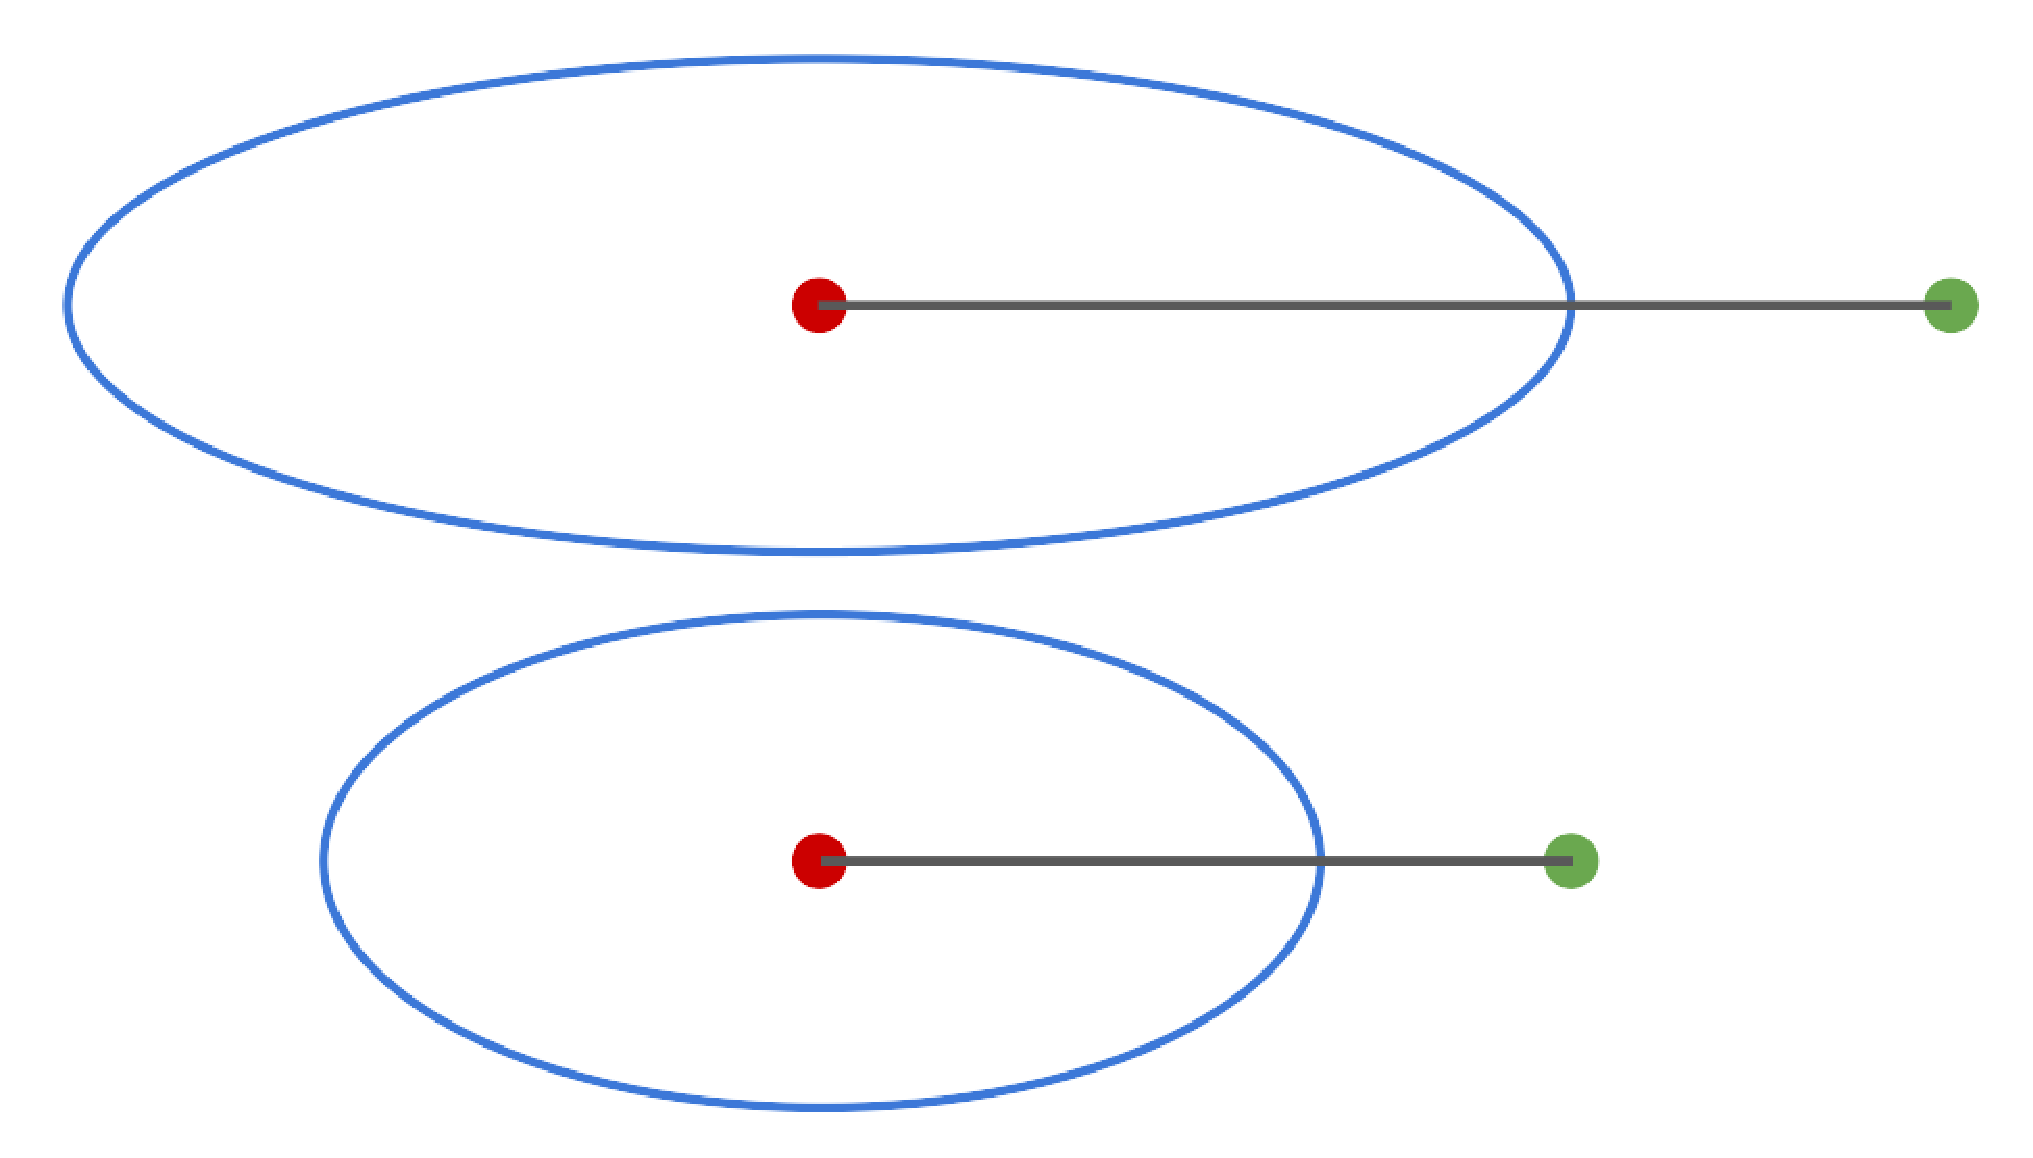
\includegraphics[width=0.5\textwidth]{images/thesis.dispdiagram.eps}
    \caption[Angular Reconstruction Disp]{The disp parameter is the angular distance between the center (red dot) of a hillas image (blue oval) and the true sky position (green dot).  Generally, longer shower images have a larger disp angle.}\label{fig:dispdiagram}
  \end{center}
\end{figure}

% https://veritas.sao.arizona.edu/wiki/index.php/BDT_Angular_reconstruction
The disp and other parameters for thousands of simulated showers can then be used to train a neural network that calculates the most probable disp for a given shower.
This most probable disp can then be used with the image axes intersection points to more accurately reconstruct the original gamma-ray point of origin.

Improved angular resolution plot??

\section{Energy Reconstruction}\label{subsec:enrecon}
A library of different showers is built, from a variety of elevations, energies, and distances from the camera.
This library can then be used to look up a real shower, find the most similar in elevation, shape, etc, and then reading that shower's library energy.


\section{Sensitivity}
% plot vs energy
Sensitivity is a measure of how difficult it is to get a signifiant detection.
It is often quantified by using simulations to predict the amount of observation time required to detect a simulated source at a given significance level.


\section{Effective Area}
% plot of effective area vs energy
Effective area is the measure of how many gamma rays a telescope can detect.
It is referred to as 'Effective' because the detection efficiency is not 100\% at all energies or all parts of the camera.
Instead it is 'effectivly' how large a detection area a telescope has, if it had perfect detection efficiency.
Different telescopes can use this number to compare roughly how many gamma rays can be detected in a given span of time.


\section{Energy Resolution}
% plot of energy resolution
Gamma rays and protons of different energies can produce similar-looking air showers.
Due to this, the reconstruction software cannot perfectly reconstruct gamma rays, which introduces errors into the different qualities of the gamma rays.
This means that when a gamma ray is reconstructed, it has a chance to be reconstructed at a lower or higher energy.
The consequence of this is that gamma rays of a given reconstructed energy can come from a distribution of true simulated energies.
Typically, simulations are run across a number of energies, and an 2D matrix is assembled, where one axis is the true simulated energy, and the other axis is bins of reconstructed energy.


\section{Point Spread Function}\label{sec:psf}
% plot of psf
In addition to the energy being slightly mis-reconstructed, the source position of the gamma ray can also be misreconstructed.
For a gamma ray telescope, a simple measure of this misreconstruction is to simulate many gamma rays at a single point in the sky, and look at how their reconstructed positions are distributed around that point.
This distribution is referred to as the Point Spread Function.
To first order, most current-generation point spread functions are gaussian distributions.


\section{Energy Dispersion}
Much like the point spread function in section \ref{sec:psf}, the energy reconstruction process is also imperfect.
This means that a gamma ray with a reconstructed energy could come from a distribution of true energies.
This can also be phrased that a group of gamma-rays with the same initial energy will have a distribution of reconstructed energies.
These distributions primarily are due to inherent randomness in the showers themselves.


\section{Energy Sensitivity and Zenith Angle}
% plot of energy sensitivity at 20zen and 65zen

As the telescope points at a lower elevation, the atmospheric volume that can be used to detect air showers greatly increases, leading to an increase in the telescope's effective areafor high energy showers.
The downside is that fewer low-energy gamma rays reach the volume of atmosphere being observed, 


\section{Comparison with Other Observatories}

% sensitivity comparison plots

CTA, HESS, Magic, HAWC, Fermi



